% Created 2018-08-29 mié 14:27
\documentclass[letterpaper]{scrartcl}
\usepackage[utf8]{inputenc}
\usepackage[T1]{fontenc}
\usepackage{fixltx2e}
\usepackage{graphicx}
\usepackage{longtable}
\usepackage{float}
\usepackage{wrapfig}
\usepackage{rotating}
\usepackage[normalem]{ulem}
\usepackage{amsmath}
\usepackage{textcomp}
\usepackage{marvosym}
\usepackage{wasysym}
\usepackage{amssymb}
\usepackage{hyperref}
\tolerance=1000
\usepackage{khpreamble}
\usepackage{subfigure}
\usepgfplotslibrary{groupplots}
\author{Kjartan Halvorsen}
\date{\today}
\title{Poles and geometric sequences exercise}
\hypersetup{
  pdfkeywords={},
  pdfsubject={},
  pdfcreator={Emacs 24.5.1 (Org mode 8.2.10)}}
\begin{document}

\maketitle


\section*{Pulse response}
\label{sec-1}
\begin{center}
\begin{minipage}[t]{0.5\linewidth}
\centering
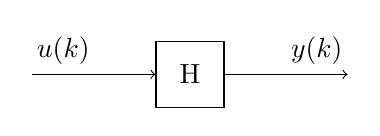
\begin{tikzpicture}[node distance=20mm, anchor=north]
\node[coordinate] (input) {};
\node[rectangle, draw, right of=input, inner sep=3mm] (lti) {H};
\node[coordinate, right of=lti] (output) {};
\draw[->] (input) -- node[near start, above] {$u(k)$}  (lti);
\draw[->] (lti) -- node[near end, above] {$y(k)$} (output);
\end{tikzpicture}
\end{minipage}
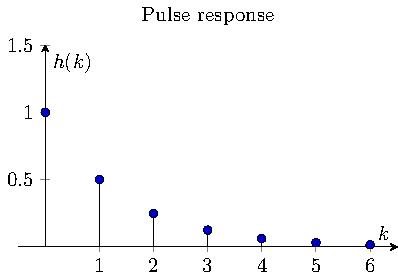
\includegraphics[0.5\linewidth]{../figures/timeplot-discrete-impulse-response}
\end{center}

\textbf{Plot the response of the system to the input signal below.}

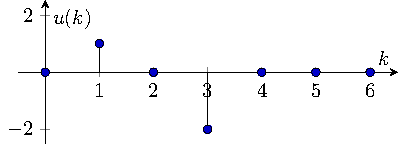
\includegraphics[0.6\linewidth]{../figures/timeplot-discrete-simplesignal}

\vspace*{1cm}

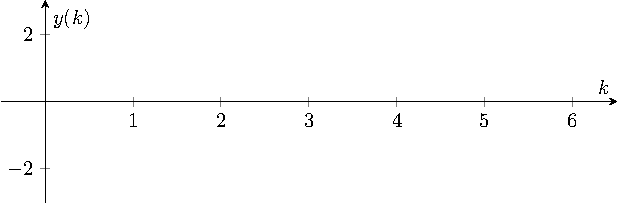
\includegraphics[0.6\linewidth]{../figures/timeplot-discrete-empty-y}



\newpage

\section*{Plot the sequence \(f(k) = a^k\) for \(k=1,2,3,\ldots\)}
\label{sec-2}

\begin{center}
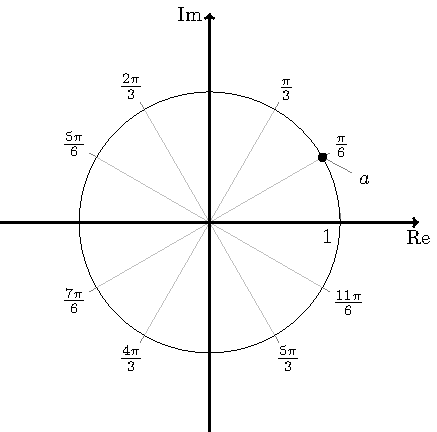
\includegraphics[width=0.38\linewidth]{../figures/imaginary-plane-seq-1}
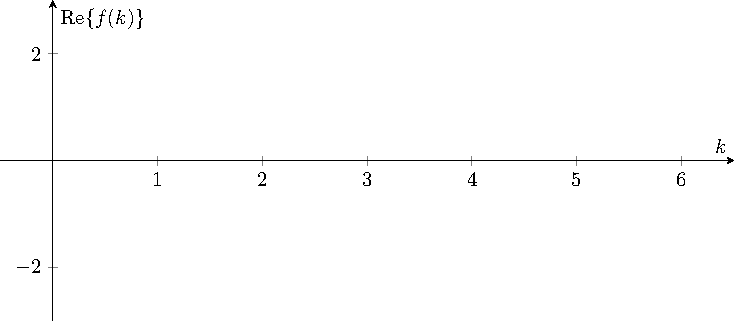
\includegraphics[width=0.6\linewidth]{../figures/timeplot-discrete-empty}\\
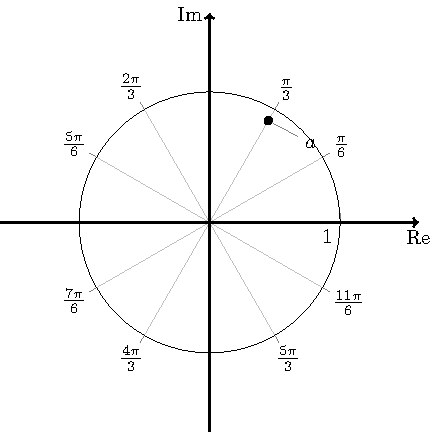
\includegraphics[width=0.38\linewidth]{../figures/imaginary-plane-seq-2}
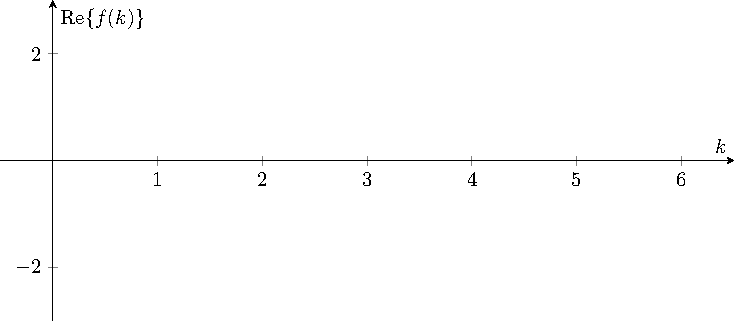
\includegraphics[width=0.6\linewidth]{../figures/timeplot-discrete-empty}\\
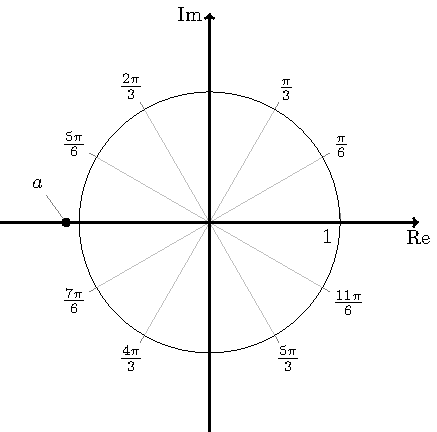
\includegraphics[width=0.38\linewidth]{../figures/imaginary-plane-seq-3}
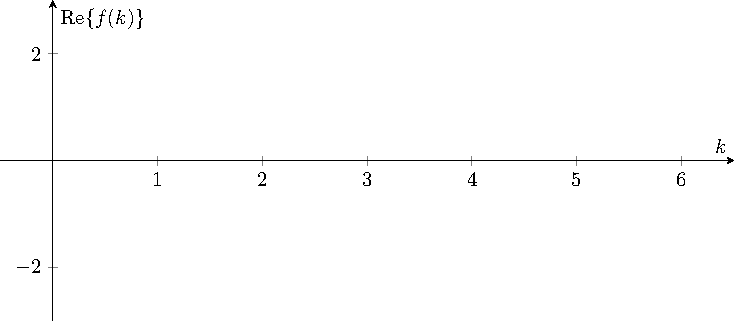
\includegraphics[width=0.6\linewidth]{../figures/timeplot-discrete-empty}\\
\end{center}



\section*{From continuous-time poles to discrete-time poles}
\label{sec-3}
\begin{center}
\begin{tabular}{cc}
\begin{minipage}[c]{0.48\linewidth}
\centering
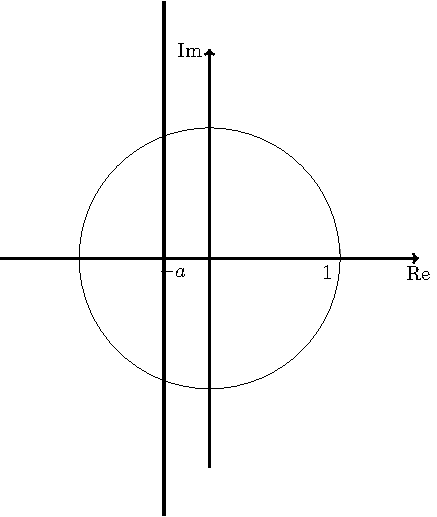
\includegraphics[width=0.8\linewidth]{../figures/imaginary-plane-vertical-line}\\
\end{minipage}
& 
\begin{minipage}[c]{0.48\linewidth}
\centering
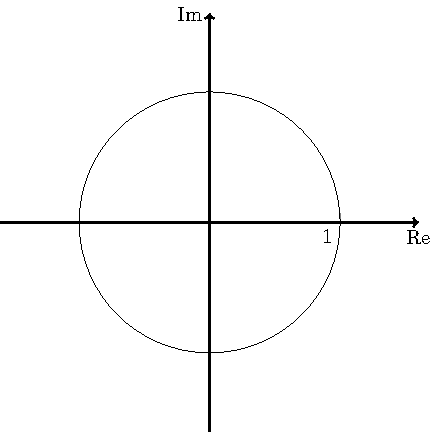
\includegraphics[width=0.8\linewidth]{../figures/imaginary-plane-empty}\\
\end{minipage} \\

\begin{minipage}[b]{0.48\linewidth}
\centering
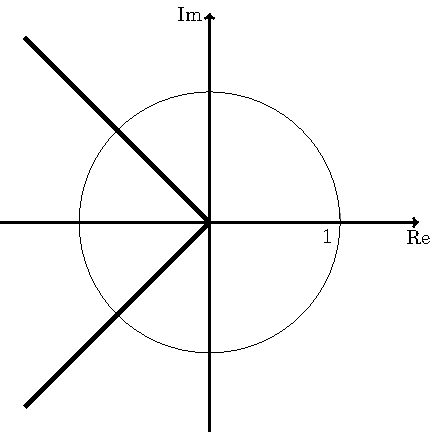
\includegraphics[width=0.8\linewidth]{../figures/imaginary-plane-diagonal-lines}\\
\end{minipage}
&
\begin{minipage}[b]{0.48\linewidth}
\centering
 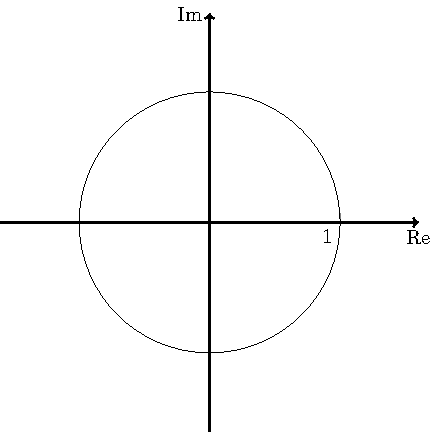
\includegraphics[width=0.8\linewidth]{../figures/imaginary-plane-empty}\\
\end{minipage}\\

\begin{minipage}[b]{0.48\linewidth}
\centering
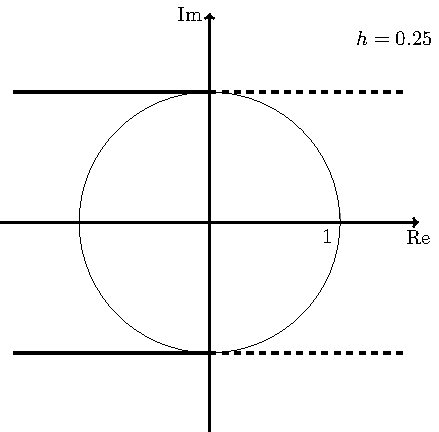
\includegraphics[width=0.8\linewidth]{../figures/imaginary-plane-horizontal-lines}\\
\end{minipage}
&
\begin{minipage}[b]{0.48\linewidth}
\centering
 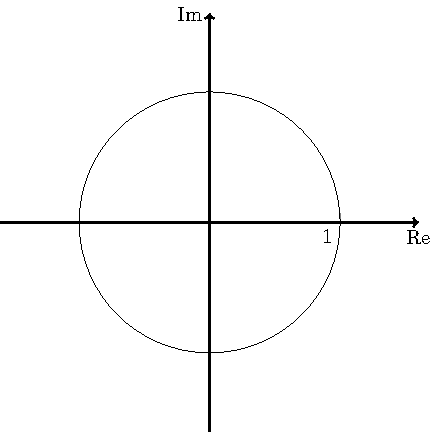
\includegraphics[width=0.8\linewidth]{../figures/imaginary-plane-empty}\\
\end{minipage}

\end{tabular}
\end{center}
% Emacs 24.5.1 (Org mode 8.2.10)
\end{document}